\section{Overview of \FW{}}\label{sect:Overview}
In this section we give an overview of \FW{} and its major components. The sections following this,  goes into detail about each individual part of the framework.

The purpose of \FW{} is to assist in functional source to target testing of ETL programs developed using pygrametl. As such, testing is performed by asserting about properties of DWs, which have been populated by an ETL program. The focus of testing lies on data loss and business rules. Testers can make assertions about new functionality or perform regression testing using old assertions. Testing is performed at the system level, meaning that the extraction, transformation and loading components have been integrated prior to test. The framework is not designed for exhaustive testing, but rather it is meant to assist in reaching an adequate level of test coverage.

\FW{} contains four major components:
\begin{itemize}
\item\textbf{DWPopulator}
\item\textbf{DWRepresentation}
\item\textbf{Predicates}
\item\textbf{Case}
\end{itemize}

The purpose of the DWPopulator is to avoid having users change their pygrametl programs for testing. ETL developers will often hardcode connections to sources and DW's into their ETL program. These contain actual data collected and used by the organization. Because of regulations such data is not available for testers to use. Thus, they have to create their own test sources and DW's. However, they should avoid having to hardcode connections to test data in their programs, as this may be time consuming and error prone. Instead, the reinterpreter allows users to dynamically insert test connections into their ETL program, when performing tests.

The DWPopulator also assists in building a DWRepresentation object from the ETL program under test. DWRepresentation is a class made to contain structural information about the DW being populated. It also allows for easy access of the DW tables and their meta data.

The Predicates are a family of classes used to make assertions about a populated DW. All of them inherit from the Predicate class. Testers make assertions by instantiating a predicate class with the tables of interest along with some other arguments depending on the predicate type. Once instantiated, a predicate can be made to check whether the defined assertion hold or not and then report upon it.

The Case is a class representing a test case, and serves as a users primary way of interacting with \FW{}. It is the class used to run a set of predicates on a DWRepresentation. It is also responsible for reporting the results of the predicates back to the users.


\subsection{Example Scenario}

\begin{figure}
\centering
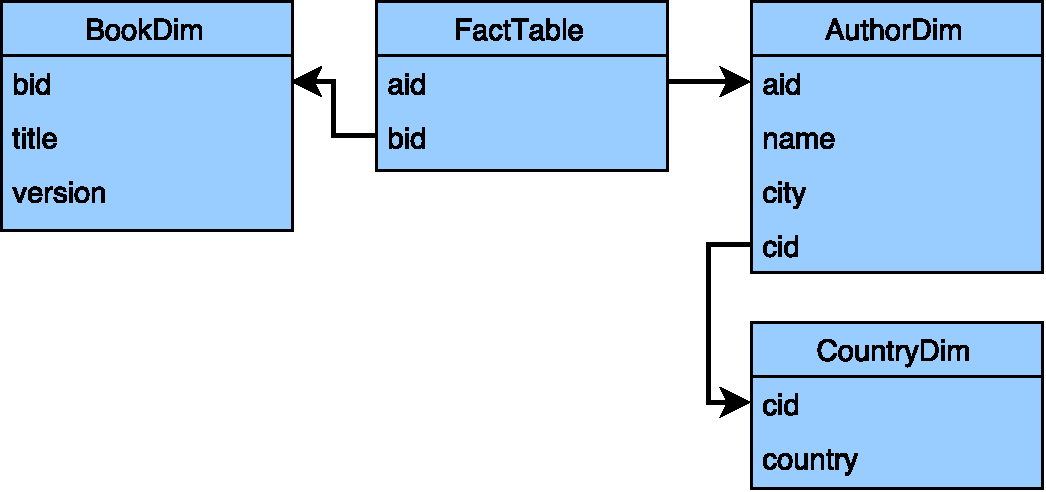
\includegraphics[width=0.48\textwidth]{figures/example_dw.pdf}
\caption{Diagram of an example DW}
\label{fig:exdw}
\end{figure}

The remainder of this section will be used to describe an example scenario, in which \FW{} is used to conduct tests. For this example we imagine that we have already written a pygrametl program which performs the necessary ETL operations to populate the DW specified by \cref{fig:exdw}. We wish to test if this pygrametl program, given two user defined sources, correctly populates the DW so that the fact table has exactly 99 rows and that there is referential integrety.
An example of a python program that does this using \FW{} can be seen in \cref{Case.py}, with an explanation of the code below.

\insertcodefile{Case.py}{Example of a \FW{} program}

\begin{description}
\item[line 5-13] In order to execute the pygrametl program with the two given sources, and to get a DWRepresentation of our DW, we use the DWPopulator. It takes as arguments the program, a pep249 module, the list of sources you wish to use, and relevant keyword arguments used for creating connections to our DW. We then call the \texttt{run} method, which returns the DWRepresentation. Note that it isn't necessary to run the DWPopulator to get a DWRepresentation, a user can simply instatiate one himself, if he already has a populated DW.
\item[line 16-18] We instantiate two predicates, one for checking if the fact table has exactly 99 rows, and one for checking if there is referential integrety in the DW.
  \item[line 21-23] We instantiate a Case, by giving the DWRepresentation and a tuple of our predicates. We then call \texttt{run} on our case, which would result in it checking if all the predicates hold and reporting accordingly. 
\end{description}


In the following sections we go into detail about the implementation of the three of the four components discussed in this section, i.e. DWPopulator, DWRepresentation and the predicates.








